\chapter{基于全局的特征提取算法}

\section{基本框架}
PCA\cite{turk1991face}是近代人脸识别中较早的方法.在文献中,作者于1991年评价了之前基于人脸手工的标定,专家模型构建的方法,并且指出了人工方法的若干不足之处.同时提出了基于统计的PCA方法,成功实现了自动的人脸识别系统.并且,作者提出了\textit{eigenface}这个用来表征人脸图像投影的空间.从那以后,研究者们从多个角度研究了许多除了\textit{eigenface}以外的方法,提出了\textit{fisherface}\cite{hsu2003practical}等一系列特征空间.

这些基于统计的方法都有着不同的出发点,但在实现上都是比较相似的.他们从不同的角度来尝试从人脸数据库中分解出更有代表性的分量,并把那些分量作为特征空间的基底.当处理新入样本时,新的样本和创建的特征空间基底作投影操作,得到的样本坐标就是该样本在空间的表示.以下是本文中所尝试的方法及其主要思想:
\begin{center}
  \footnotesize
  \begin{tabular}{l|c}
  \hline 
    方法 & 主要思想 \\ \hline
    PCA & 在假设样本高斯分布的情况下,寻找样本空间特征值最大的k个正交向量作为基底\\ \hline
    NMF & 由于图片仅由正实数表示,提出了保证特征向量也为正数的前提下的特征分解方法\\ \hline
    ICA & 在假设样本独立统计(I.I.D)及非高斯分布的情况下,来近似估计各个独立分量成分\\
    \hline
  \end{tabular}
      \captionof{table}{本文中所尝试的降维方法及其主要思想}
\end{center}
\subsection{人脸分解的例子}
下面以PCA为例,来表示一个具体的基于全局的人脸特征提取算法的工作流程.
\paragraph{构建基底空间} 这一步骤是不同方法的主要区分之处,不同的算法主要是从不同的角度来构建更为优化的投影空间,使得投影后的样本坐标更具有表现力.
\newline
下面是通过分解ORL数据库所有图片得到的前6张特征脸(\textit{eigenfaces})和平均脸:

\begin{center}
\begin{minipage}[t]{\linewidth}
%\label{fig:main}
\center
{
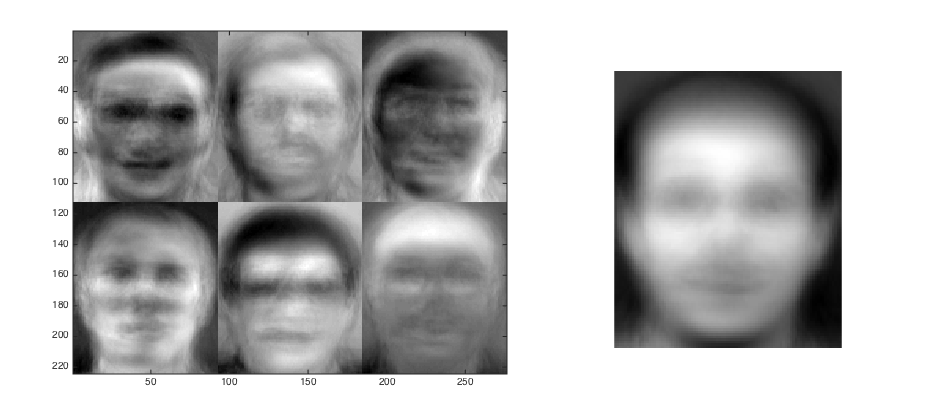
\includegraphics[width=\MyFactor\textwidth]{Img/pca_eigenspace.png} \captionof{figure}{前6张特征脸和平均脸}
}
\end{minipage}
\medskip
\end{center}

其中,PCA的计算在给出特征向量的同时,还会给出代表特征向量权重的特征值,上述6个特征值在400个特征向量空间中占据了51.4\%的权重.权重分布如下图:

\begin{figure}[!htbp]
\centering 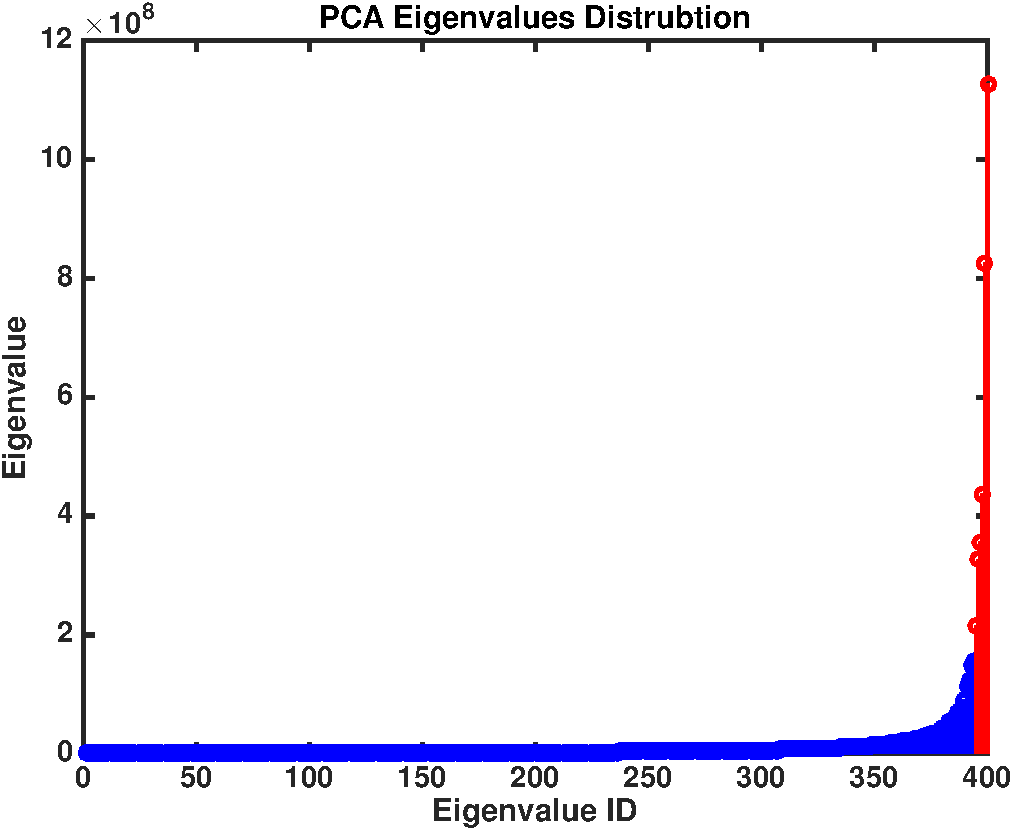
\includegraphics[width=\MyFactor\textwidth]{Img/pca_eivalue.pdf} 
\caption{特征值分布图 \\ 蓝色:舍弃的特征向量, 红色: 保留的特征向量}
\end{figure}
设特征向量组成的基底矩阵为V, 输入图像为I, 则该步骤可以表示为:
\begin{equation}
Weights = Inv(V) \cdot I
\end{equation}
其中
\begin{itemize}
	\item V为一个$m  \times  n$的矩阵,m是特征脸的像素数,n是特征向量的数目,$Inv(V)$为其转置矩阵
	\item I为一个$m \times d$的矩阵,m是特征脸的像素数,d是需要分解的输入图像数目
	\item Weights为一个$n \times d$的矩阵,n是特征向量的数目,d是需要分解的输入图像
\end{itemize}


本例中图像在特征向量空间下的权值如下:
\begin{center}\begin{tabular}{|l|l|l|l|l|l|}
\hline
-123.7915&-689.9194&261.7842&1867.0258&1072.1813&1531.176\\\hline
\end{tabular}
\end{center}

\paragraph{输入样本重构} 这一步是根据上一步求得的权值来线性地重构这张输入样本.当然了,当实际应用时不需要恢复原始输入图片时,这一步可以省略.

\begin{center}
\begin{minipage}[t]{\linewidth}
%\label{fig:main}
\center
{
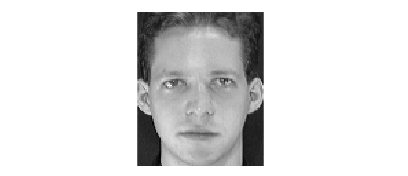
\includegraphics[width=\MyFactor\textwidth]{Img/pca_sample.png} \captionof{figure}{左:输入图像 右:重建后的图像}
}
\end{minipage}
\medskip
\end{center}

	
	以下是该流程的简要示意:
\begin{center}
\begin{minipage}[t]{\linewidth}
%\label{fig:main}
\center
{
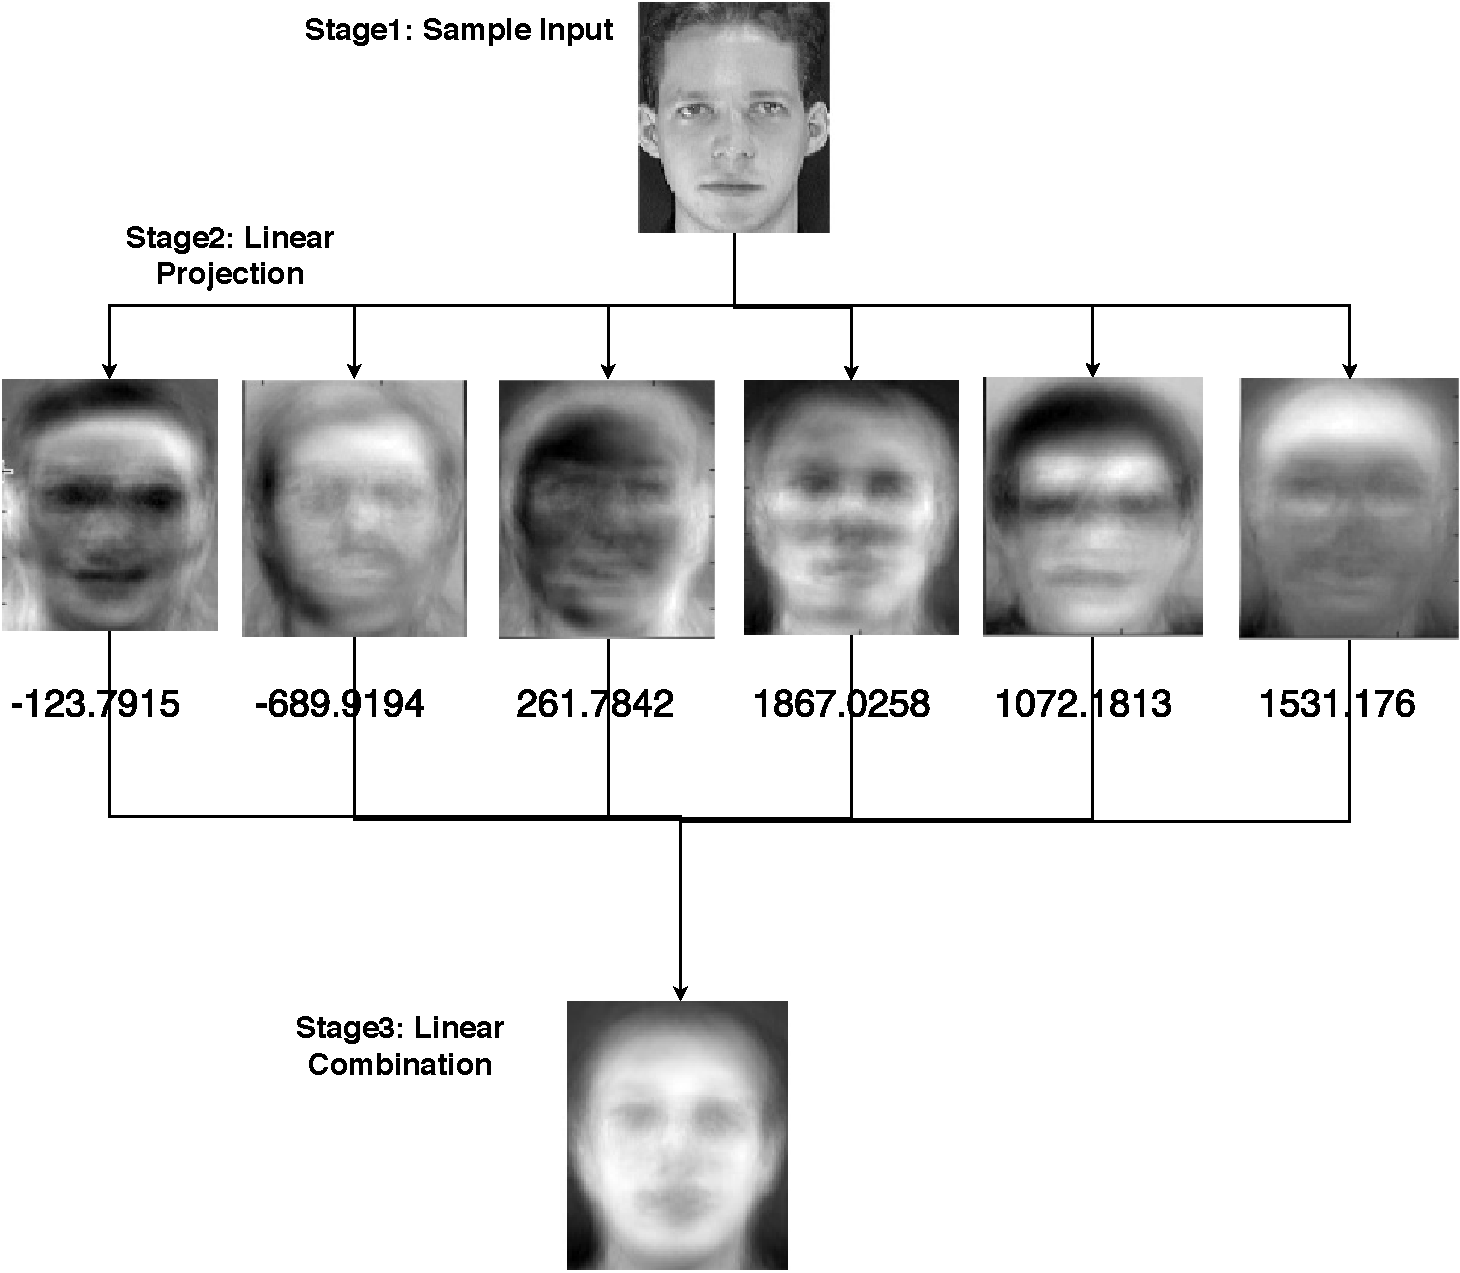
\includegraphics[width=0.8\textwidth]{Img/pca_demo.pdf} 
\captionof{figure}{图像投影示意}
}
\end{minipage}
\medskip
\end{center}

\subsection{两类不同的特征空间}
\begin{center}
\begin{minipage}[t]{\linewidth}
%\label{fig:main}
\center
{
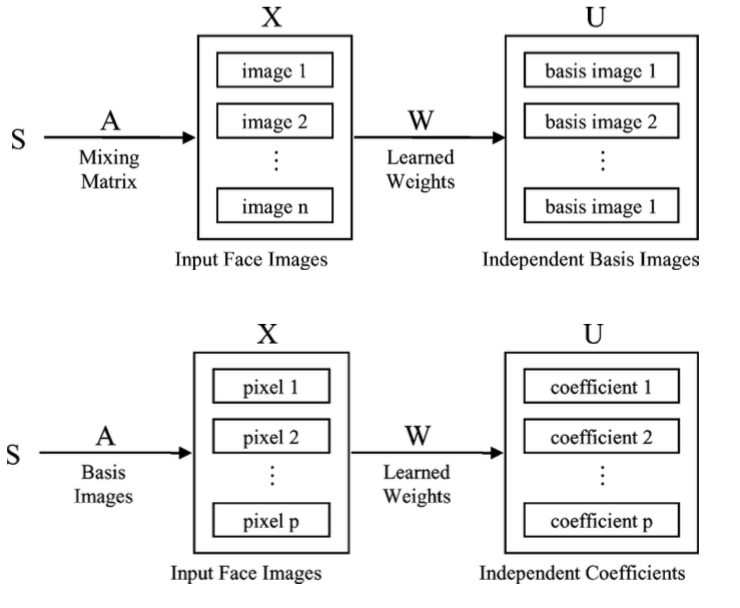
\includegraphics[scale=1]{Img/ica_c1c2.png} 
\captionof{figure}{图像投影示意 \\ 上: Architecture I, 下: Architecture II. 来源\cite{draper2003recognizing}}
}
\end{minipage}
\medskip
\end{center}
值得指出的是,受到\cite{draper2003recognizing}启发.这里同时存在着两类不同的分解思想.他们的区别在于一类的输入样本是另一类的转置.\\



第一类的思想是将人脸图像作为变量而将每张图像上的像素作为这个变量的描述,而分解的操作发生在人脸的空间上.


第二类的思想是将人脸图像样本作为各个像素的描述,并且转而把像素作为变量.
\\
在实践中由于第二类的维数过高,运算量太大,采用了第一类.\todo{ArchitectureII}
\section{PCA}
本章节的主要依据文献是\cite{turk1991eigenfaces}和\cite{turk1991face},从本章节开始,将依次简要介绍PCA, NMF, ICA的基本原理和计算方法.并在ORL数据库下给出其特征脸空间. \newline

根据\cite{de2010face}和\cite{smith2002tutorial},当PCA的运算数据中减去其平均值(又称为平均脸),PCA运算等价于KL运算.所以本文也是对KL运算的介绍.\newline

\subsection{PCA的思想}
\begin{enumerate}
	\item 记$\tau_i$为由第i张基底计算集图像形成的图像.原始图像是一个$m \times n$大小的矩阵,$\tau$为一个原始图像按照行展开形成的$ m \times n$长的行向量
	\item 记\begin{equation}\Phi = \frac{1}{M}\Sigma_{n-1}^M\tau_n\end{equation}$\Phi$是$\tau_i$的平均值,也就是这个基底计算集的平均脸,M是基底计算集的样本数目
	\item 记\begin{equation}\phi_i = \tau_i - \Phi\end{equation}
	\item PCA旨在选择值最大的若干$\lambda$,\begin{equation} \lambda_k = \frac{1}{M}\Sigma^M_{n=1}(u^T_k \phi_i)^2\end{equation} 同时,$u_k$受到正交性的限制:\begin{equation} u_k \times u_l = \left\{\begin{array}{c}
        1(k = l)\\
        0(k \neq l)
    \end{array}\right.
    \end{equation}其中$\lambda$被称作特征值,$u$被称作特征向量,也就是所求的特征基底.
	\item $\lambda_k$的个数是需要选择的,选择的特征向量数越多,保留的内容就越多,但同时压缩效果就越差
\end{enumerate}
\subsection{PCA的计算方法}
从线性代数的角度,PCA相当于最小化这个样本集的二阶统计值,当PCA完成后,各个特征向量之间的相关性为0.而$u$,$\lambda$分别为相关矩阵C的特征值,特征向量.
\begin{equation}
	C = A \cdot A^T
\end{equation}
A是样本集,也就是$[\phi_1, \phi_2,...,\phi_M]$\\ 

由于C为一个$(m \times n) \times (m \times n)$大小的矩阵,直接计算不便,经分析,对C的计算等价于对L的计算,L定义为
\begin{equation}
	L = A^T \cdot A
\end{equation}
L是一个$M \times M$大小的矩阵.
而计算过程也就是计算L矩阵的特征向量,特征值.而此时的特征向量$v$并非直接可用的向量,其大小为$M \times M$,而选择过k个特征值最大的的向量后,其大小为$M \times k$,需要使用计算
	\begin{equation}
		u=A \cdot v
	\end{equation} 
	便得到了大小为$(m \times n) \times k$的特征基底.
\subsection{PCA的在ORL测试集的投影基底}
以下是使用ORL数据集400张图片作为基地,选择特征值最大的前64张图片得到的特征基底.
\begin{center}
\begin{minipage}[t]{\linewidth}
%\label{fig:main}
\center
{
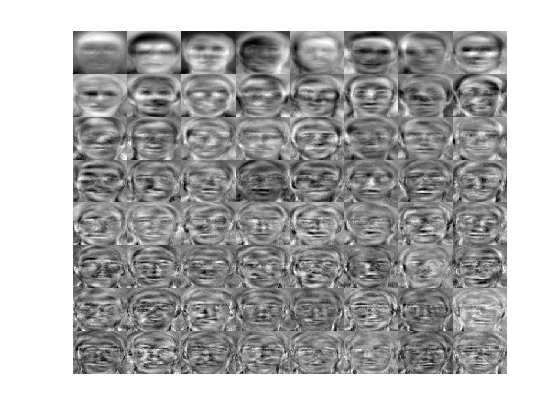
\includegraphics[width=\textwidth]{Img/pca_base.png} \captionof{figure}{PCA的在ORL测试集的投影基底}
}
\end{minipage}
\medskip
\end{center}

\section{NMF}

\section{NMF的思想和计算方法}
本章节的内容主要基于\cite{lee1999learning}和\cite{lee2001algorithms}.\newline

NMF算法围绕着在保证分量非负性的同时达到$V=W \cdot H$的分解.其中的V与等价于上一章节的$[\tau_1, \tau_2,...\tau_M]$,是基底计算样本的全集. NMF定义了惩罚函数\begin{equation}||V-W\cdot H|| = \Sigma_{ij} = (V_{ij} - WH_{ij})^2\end{equation}来描述分解的效果.$||V-W\cdot H||$是V和WH之间的欧式距离.实现完全分解时$||V-W\cdot H||=0$

NMF算法提出了保证W,H非负性的前提下的迭代公式,并证明了其收敛性,使用迭代的方法来逐步逼近最终的W,H.其迭代公式如下
	\begin{equation}
		H_{au} = H_{au}\frac{(W^TV)_{au}}{(W^TWH)_{au}}
	\end{equation}
	\begin{equation}
		W_{ia} = W_{ia}\frac{(VH^T)_{ia}}{(WHH^T)_{ia}}	
	\end{equation}
可以看到H,W的迭代运算中使用的仅仅是除法,乘法和加法,而同时V矩阵初值均为正数这就保证了H,W的非负性.\newline

同时,需要注意的是
\begin{itemize}
	\item 上述的迭代公式并非全局最优解.对于$||V-W\cdot H||$这个优化函数,目前并没有可以同时优化W和H的方法.NMF方法采用的是迭代的方法,也就是,优化H时,以上一步的W为目前最佳W,优化W时,以上一步的H为目前最佳H.而其该局限性使得这种优化方法只能收敛到局部最小值\cite{berry2007algorithms}.
	\item 上述的迭代公式,惩罚函数只是NMF思想的一种实现方式.现实中还有其他的替代方法.在\cite{lee1999learning}和\cite{lee2001algorithms}就列写了另一个惩罚函数和对应的迭代公式,还有对应迭代公式收敛性的证明.其惩罚函数为$$\Sigma_{ij}A_{ij} log \frac{A_{ij}}{B_{ij}} - A_{ij} + B_{ij}$$
\end{itemize}

\subsection{NMF的终止条件}
\subsection{本项目NMF投影空间}

\section{ICA}

\subsection{ICA的不同实现方法}


\subsection{本项目ICA投影空间}
\subsection{ICA的其他应用}
同时,需要指出的,ICA的分解结果有很强的稀疏性,因此也被用来做图像压缩的算法.
\subsubsection{分块ICA用于图片压缩}

\section{DCT}
\subsection{DCT的原理}
\section{更多的基底}
除了这些方法,还有很多其他的方法.\cite{de2010face}列出了更为详尽的列表,限于项目时间的限制,并没有深入研究这些所有的算法,仅仅尽可能的通过\textit{SciKit}工具包来列出相同测试样本下的基底.
	\begin{itemize}
		\item Kernel PCA
		\item Weighted PCA
		\item Linear Discriminant Analysis (LDA)
		\item Kernel LDA
		\item Semi-supervised Discriminant Analysis (SDA)
		\item Neural Network based methods
		\item Multidimensional Scaling (MDS)
		\item Self-organizing map (SOM)
		\item Active Shape Models (ASM)
		\item Active Appearance Models (AAM)
		\item Gavor wavelet transforms
		\item MMSD, SMSD
	\end{itemize}
\section{实验:数据的低维表示}

